\documentclass{article}

\usepackage{amsmath, amssymb}
\usepackage{amsthm}
\usepackage{graphicx}
\usepackage[top=1in, left=1in, right=1in]{geometry}
\usepackage{enumerate}
\usepackage{color}   %May be necessary if you want to color links
\usepackage{hyperref}
\hypersetup{
    colorlinks=true, %set true if you want colored links
    linktoc=all,     %set to all if you want both sections and subsections linked
    linkcolor=blue,  %choose some color if you want links to stand out
}
\newcommand\Carrat{\mathbin{\char`\^}}
\usepackage{fancyhdr}

\lhead{Marco Salazar, Dishaan Ahuja, Donggu Kang }
\rhead{salazarm, dishaan, donggu}
\title{Midipiano Documentation }

\pagestyle{fancy}

\begin{document}
\setlength{\headheight}{24pt}

\section{Lexer and Tokens}
 Lexer takes a string representation of an ABC file (extracted through our main method) and creates tokens out of it. It first parses the header and then parses the body. It has 2 methods that return an ArrayList of Tokens for header and body respectively. The tokens are any of the following:\\ \\
\texttt{
		ACCIDENTAL, BASENOTE, CHORDSTART, CHORDEND, NOTEMULTIPLIER, 
		BARLINE, REST, REPEATSTART,\\ REPEATSECTION, REPEATEND, TUPLET, VOICE,
		COMPOSER, TITLE, INDEX, KEY, METER, TEMPO, \\NOTELENGTH, ENDMAJORSECTION, OCTAVE
		}
\\ \\
We used a for loop to iterate over the string and matched the remainder of the string to a pattern corresponding to one of these tokens. This made it easy to go through the whole string without using too many conditional statements besides the regular expressions.
\section{Parser}
{\tt Parser} is instantiated with a {\tt Lexer} in it's constructor and within the constructor it generates a header object and a body object. By calling the {\tt parseBody} and {\tt parseHeader} methods a Player object is created from the body and header object and is returned by the {\tt Parser}. The {\tt parseBody} method first determines whether there were voices supplied in the abc file, if not it will create a default {\tt  Voice}. It then goes through the {\tt Token} objects calling the appropriate methods to parse the {\tt Token} objects and it assigns it to the current {\tt  Voice }which is the last seen {\tt Voice}. Below is a diagram illustrating our {\tt Parser} as a state machine.
\begin{figure}[htbp]
\centering
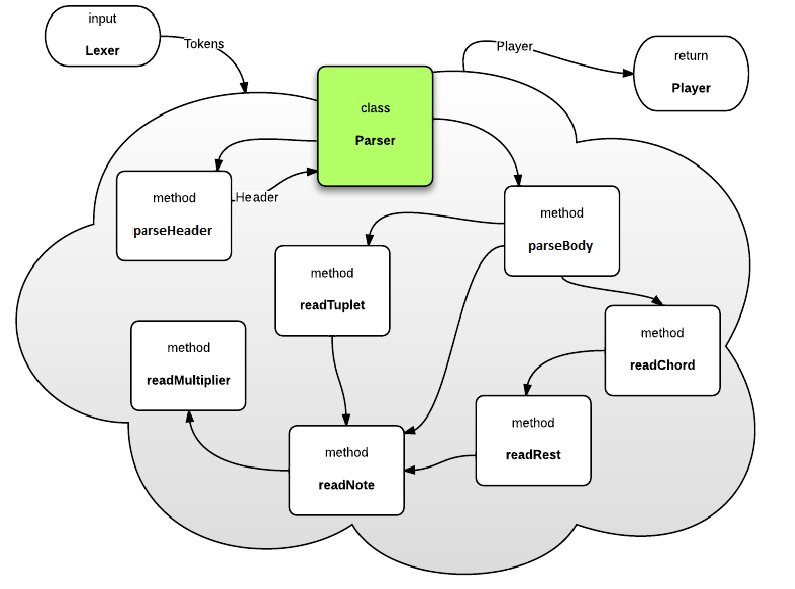
\includegraphics[width=.7\textwidth]{C:/Users/DW/workspace/dishaan-salazarm-donggu/abcPlayer/Documents/ParserDiagram}
\caption{}
\label{fig:ParserDiagram}
\end{figure}




\section{Datatypes}
\subsection*{ {\tt public enum KeySignature: KeySignature(int[] keyAccidentals, String stringRep)}}
Representation of key signature types. The {\tt keyAccidentals} array keep track of which {\tt Notes} need to be transposed for a particular key signature, while {\tt stringRep} contains a {\tt String} representation of the name of the key signature in abc. it contains getter methods for {\tt keyAccidental} objects, {\tt stringRep}, and the {\tt keyAccidental} type.
\subsection*{{\tt public class Accidental: public Accidental(int intRep)}}
Represents an accidental to be applied to a {\tt Note}. {\tt intRep} is the integer representation of the transposition of pitch by the {\tt Accidental}.
\subsection*{{\tt public class Fraction: pulic Fraction(int numerator, int denominator)}}
This class represents a {\tt Fraction}, to be used to store the meter and default note length. It has the following attributes:
\begin{itemize}
\item {\verb int numerator} - Numerator of Fraction.
\item {\verb int denominator} - Positive denominator of Fraction.
\end{itemize}
\subsection*{{\tt public abstract class MusicSequence:}}
This class represents a valid musical construct of an abc file. It includes an accept() method for visitors that wish to perform operations on a particular {\tt MusicSequence}. It includes a {\tt startTick} attribute and getter and setter methods for this attribute.
\subsection*{{\tt public class Note extends MusicSequence: \\ public Note(char baseNote, int octaveMOdifier,\\ Accidental accidentalModifer, double NnoteMultiplier)}}
This class represents a not in an abc file using the following attributes:
\begin{itemize}
\item {\tt char baseNote} - Represents the base note of the {\tt Note}.
\item {\tt int octaveModifer} - Represents the particular type of {\tt Accidental} applied to this {\tt Note}
\item {\tt Accidental accidentalModifier} - Represents the particular type of {\tt Accidental} applied to this {\tt Note}.
\item {\tt Pitch notePitch} - {\tt Pitch} object created with the above parameters
\item {\tt double noteMultiplier} - Represents a multiplier for the length of the {\tt Note}, a multiplier of 1 indicates that the {\tt Note} is of default length as specified in the header.
\end{itemize}
This class includes getter methods for the above fields as well as an {\tt accept() } method for visitors.
\subsection*{{\tt public class Rest extends Music Sequence: public Rest(noteMultiplier) }}
	This class represents a rest in an abc file. It has one attribute: the {\tt  noteMultiplier}, which acts similarly to the {\tt noteMultiplier} in the {\tt Note} class.
\subsection*{{\tt public class Chord extends MusicSequence: \\
			public Chord(List<Note>notes)}}	
This class represents a chord in an abc file. It hast the following attributes:
\begin{itemize}
\item {\tt  List<Note> notes} - Represent the {\tt Notes} that make up the chord.
\end{itemize}
This class includes getter methods for the above fields, as well as an {\tt accept()} method for visitors.
\subsection*{{\tt public class Tuplet extends MusicSequence: public Tuplet(List<Note> notes)}}
\begin{itemize}
\item {\tt  int tupletNumber} - Represents the type of tuplet $\in (2,3,4)$
\item {\tt  List<Notes> notes } - Represents the {\tt Notes} to apply the tuplet to
\end{itemize}
This class includes getter methods for the above fields, as well as an {\tt accept() } method for visitors and a method to increment the current tick, as well as to get the current tick.

\subsection*{{\tt public class Voice extends MusicSequence: public Voice(String voiceName)}}
This class represents a voice in an abc file. It has the following attributes:
\begin{itemize}
\item {\tt String voiceName} - Name of the {\tt Voice}
\item {\tt List<MusicSequence> musicSequences - MusicSequence} objects that compose this {\tt Voice}.
\end{itemize}
This class has getter and setter methods for these attributes, as well as methods to handle {\tt Repeats}. It also contains methods to get and increment the current tick.

\subsection*{{\tt public class Body extends MusicSequence: public Body()}}
This class contains an {\tt ArrayList} of {\tt Voices} that make up the body of the abc piece. If no voice names are mentioned in the header, the list contains only one (default) {\tt Voice}. It contains the following attributes:
\begin{itemize}
\item {\tt List<Voice> voices} - List of voices present in the body of this abc piece. If no voice names are mentioned in the header, the list contains only one (default) {\tt Voice}.
\end{itemize}
It contains methods to add the {\tt ArrayList} of voices, to get the {\tt ArrayList} of {\tt Voice} objects, and an {\tt accept()} method for visitors.

\subsection*{{\tt public class Header: public Header(int indexNumber, String title, KeySignature keySignature)}}
This class contains the header information that is included in every abc file. It has the following attributes:
\begin{itemize}
\item {\tt String composer} - Name of the composer of the piece, default value "Unknown" represents the "C" field in the header.
\item {\tt int title} - Title of the piece, mandatory argument to the constructor as per abc specifications. Represents the "T" field in the header.
\item {\tt int temp} - Represents the number of default-length notes per minute. Default value is 100. Represents the "Q" field in the header.
\item {\tt Fraction defaultNoteLengthFraction} - Default duration of a note in this piece, default value set to $\dfrac{1}{8}$. The value is represented as a {\tt Fraction} to preserve the numerator and denominator so the header can be faithfully printed by the {\tt abcPlayer}. Represents the "L" field in the header.
\item {\tt KeySignature keySignature} - Key signature of the piece, mandatory argument to the constructor. Represents the "K" field in the header.
\item {\tt Fraction meter} - Represents the sum of all durations within a bar. Represents the "M" field in the header.
\item {\tt List<String> voices} - Represents the name of the voices in the piece. Represents the "V" fields in the header.
\end{itemize}
This class includes getter and setter methods for the above fields, as well as overridden {\tt toString()} method.

\subsection*{{\tt public class Player: public Player(Header header, Body body)}}
This class contains a {\tt SequencePLayer} that plays the {\tt MusicSequence} objects contained within the {\tt Body}. The {\tt Header} and {\tt Body} attributes are passed to the constructor while the {\tt beatsPerMinute} and {\tt ticksPerQuarterNote} attributes are calculated from information in the {\tt Header}. It includes getter methods for these attributes, as well as methods to schedule and play the {\tt Body"}.

\subsection*{{\tt public interface Visitor<R>:}}
This class represents a generic visitor for a {\tt MusicSequence}. It contains methods corresponding to each type of {\tt MusicSequence}.

\subsection*{{\tt public class Duration implements Visitor<Integer>: public Duration(Player player)}}
This class uses the Visitor design pattern to calculate the duration of varius types of {\tt MusicSequence} objects in the given player.

\subsection*{{\tt public class MusicSequenceSchedule implements Visitor<Void>:\\ public MusicSequenceScheduler(Player player)}}
This class uses the Visitor pattern to schedule {\tt MusicSequence} objects in the supplied {\tt Player}.


\section{Design Decisions}	
	\begin{itemize}
	\item[1] We chose not to have a \texttt{DOUBLESHARP} or \texttt{DOUBLEFLAT} {\tt token}; instead we had these operations on \texttt{NOTE} taken care of by the {\tt parser}
	\item[2] We implemented the visitor pattern to handle both the duration and scheduling of our {\tt MusicSequence}
	\item[3] We chose not to check for incomplete measures.
	\item[4] Even when there is no {\tt Voice} specified in the header, we use a default {\tt Voice}. This allows us to have one general implementation for all {\tt abc} files.
	\item[5] We added a {\tt Fraction} datatype to represent te meter and default note length.\
	\end{itemize}
\section{Grammar}
	{\tt
	abcFile ::= abcHeader abcBody\\
	abcHeader ::= fieldNum title comment* optionalFields* key\\
	fieldNum ::= "X:"[0-9]+ end\\
	title ::= "T":" text end\\
	key: ::= "K:" baseNote('\#'|'b')?('m')? end\\
	optionalFields ::= composer | noteLength | meter | tempo |voice | comment\\
	composer ::= "C:" text end\\
	noteLength ::= "L:" fraction end\\
	meter ::= "M":" ("C"|"C|"|fraction) end\\
	tempo ::= "Q:"[0-9]+ end\\
	voice ::= "V:" text end\\\\
	abcBody ::= line+\\
	line ::= (element* endOfLine) | voice | comment\\
	nonBar ::= noteRep | tuplet| repeat| space \\
	element ::= |? nonBar |?\\
	noteRep ::= note | chord\\
	chord ::= "["note+"]"\\
	note ::= noteType(noteMultiplier)?\\
	noteType ::= pitch | rest\\
	noteMultiplier ::= ([0-9]*)("/"[0-9]*)?\\
	rest ::= "z" (noteMultiplier)?\\
	pitch ::= (accidental)?baseNote(octave)?\\}
{\tt accidental ::= "\^{ } "|"\^{ }\^{ } "|"="|"\_"|"\_\_" } \\
	{\tt baseNote ::= [a-gA-G]\\
	octave ::= "'"+|"."+\\
	tuplet ::= "("[2-4]noteRep+\\
	repeat ::= repeatSimple| repeatAlternate\\
	repeatSimple ::= (repeatStart noteRep+(barline noteRep+)* repeatEnd)\\
	repeatAlternate ::= ( repeatStart  noteRep+ (barline noteRep+)* “[1”\\ noteRep+ (barline noteRep+)* “[2” noteRep+ repeatEnd)\\
	barline ::= “|”\\
	repeatStart ::= “|:”\\
	repeatEnd ::= “:|”\\
	majorEnd ::= “||” | “|]”\\
	text ::= [.]\\
	newLine ::=  "$\backslash$n" \\
	space ::= " " | "$\backslash$t" \\
	comment ::= “\%” text endOfLine\\
	end ::= endOfLine | comment\\
	endOfLine ::= newline | endOfFile\\
	}
\section{Revisions}
\begin{itemize}
	\item[1] We decided to make {\tt MusicSequence} an Abstract Class rather than an interface so that we can could implement the {\tt getTick() } and {\tt setTick }methods.We
	\item[2] We decided that { \tt Voice }should extend {\tt MusicSequence} because it contains {\tt MusicSequence}.
	\item[3] We added a {\tt Body} class that contained all of our {\tt MusicSequence} as opposed to having the player store an {\tt ArrayList} of {\tt MusicSequences}
	\item[4] We made {\tt KeySignature} an {\tt enum} type rather than a class because all {\tt KeySignature} are constant and have specific attributes that we need to query efficiently; and an {\tt enum} type is much better suited for this than a class. (This functions similarly to a hash map).
	\item[5] We modified the definition of {\tt element} in the Grammar so that two bar lines without any {\tt MusicSequence} in between would be prohibited.
	\item[6] We corrected the definition of {\tt repeat} in the Grammar.
	\item[7] We separated the definition of a{\tt barline} from {\tt repeatEnd},{\tt repeatStart}, and {\tt majorEnd}.
	\item[8] {\tt Note} is no longer an interface and is instead a class that extends {\tt MusicSequence}; this also means that {\tt Rest} is a separate concrete implementation of {\tt MusicSequence}. Additionally the {\tt Pitch} class extending {\tt Note} has been deprecated in favor of storing the pitch as an attribute in {\tt Note} itself.
	\item[9] Removed the {\tt Repeat} class and had the {\tt Voice} class handle repeats because we needed access to the {\tt MusicSequence} objects that came prior to the repeat in the {\tt Voice} class in case we had to start the repeat from a different section.
\end{itemize}

\end{document}